\subsubsection{Antlr}\label{subsubsec:antlr}
\ac{Antlr} bietet die Möglichkeit einen Parser über eine eigens geschriebene Grammatik zu generieren.
Die Grammatik muss linksableitend sein und ist in erweiterter Backus-Naur-Form definiert.
Der generierte Parser ermöglicht zudem das Aufbauen und Ablaufen eines~\textit{Parse trees}.
Bei einem~\textit{Parse tree} handelt es sich um einen Syntaxbaum, in welchem über eine hierarchische Struktur ein Text in mehrere Knoten unterteilt wird.
Hierdurch ergibt sich die Möglichkeit, während dem Parsen weitere Aktionen durchzuführen, welche den späteren Programmablauf eines Tools unterstützen können.

\begin{listing}[!ht]
    \inputminted{antlr-java}{listings/2.2.1/AntlrExample.g4}
    \caption{Beispiel einer einfachen Grammatik in \ac{Antlr}}
    \label{listing:grammar-example}
\end{listing}

In Listing~\ref{listing:grammar-example} ist ein Beispiel für eine einfache Grammatik zur Erkennung von Wertzuweisungen beziehungsweise dem Erstellen von
Properties dargestellt\cite*{antlrOrg}.
Es existieren drei nicht-terminale Regeln, welche für den generierten Parser wichtig sind, und den Gesamtaufbau einer Eingabe definieren.
Die Grammatik kann mehrere Properties verarbeiten, welche aus einer ID, einem Gleichheitszeichen und einem Wert bestehen.
Hierbei ist in Zeile 4 zu erkennen, dass nach jeder Property eine neue Zeile begonnen werden muss.
Ein Wert kann entweder ein String oder eine ID sein.
\textit{STRING} und \textit{ID} sind terminale Regeln, welche einen finalen Knoten für einen Ast des Parse Trees darstellen.
Eine zulässige Eingabe für die festgelegte Grammatik aus Listing~\ref{listing:grammar-example} ist in Listing~\ref{listing:prop-input} dargestellt.

\begin{listing}[!ht]
    \begin{minted}{text}
name=parrt
title="Supreme dictator for life"

    \end{minted}
    \caption{Eingabe}
    \label{listing:prop-input}
\end{listing}

Die zuvor beschriebene Grammatik kann mittels weiterer Tools auf eine Eingabe geprüft werden.
Eines dieser Tools ist das \ac{Antlr}-Plugin für~\textit{IntelliJ}.
Die Überprüfung auf die Richtigkeit einer Eingabe oder auch der Grammatik kann über das Plugin bereits vor einer Generierung von Code durchgeführt werden.
Weiterhin ist es möglich einen Parse Tree zu generieren, was in Abbildung~\ref{fig:parse-example} betrachtet werden kann.

\begin{figure}[h]
    \centering
    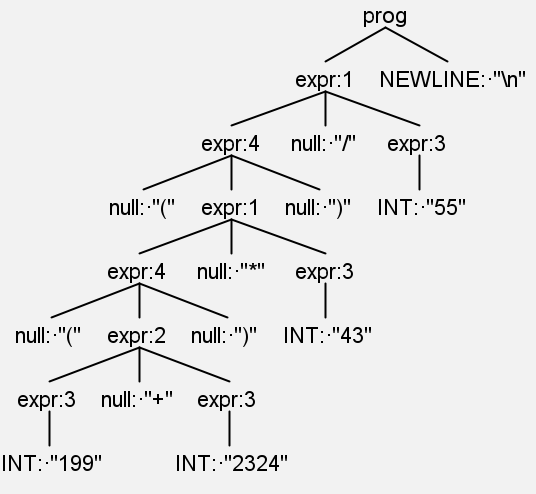
\includegraphics[width=0.5\textwidth]{images/2.2/parseTreeExample}
    \caption{Interner Parse Tree}
    \label{fig:parse-example}
\end{figure}

Hierbei ist ersichtlich, dass die Wurzel bei der obersten Regel~\textbf{file} beginnt und alle weiteren Kindknoten durch \textbf{prop} Regeln kreiert wurden.
Beide Properties besitzen eine ID und einen Wert, welcher durch ein Gleichheitszeichen und einen Zeilenumbruch umklammert ist.
Der zugeordnete Wert ist bei den Properties dieses Beispieles allerdings unterschiedlich in \textit{ID} und \textit{STRING} aufgeteilt.
Dies entsteht durch die Unterscheidung bei der Grammatik in Terminale und Nicht-Terminale.
Hierbei werden wie in Listing~\ref{listing:grammar-example} dargestellt nicht-terminale Regeln kleingeschrieben und terminale Regeln werden in Großbuchstaben verfasst.
In der vereinfachten Grammatik sind lediglich ganze Zahlen als Eingabe erlaubt.

Dies sind einzig die Grundlagen von \ac{Antlr}, auf die genauere Verwendung des generierten Parsers und Besonderheiten der Grammatik wird in Kapitel~\ref{subsec:antlr-grammatik},
anhand der Implementierung, eingegangen.
